\documentclass{beamer}
%\documentclass[handout]{beamer}

%\setbeamertemplate{background canvas}[vertical shading][bottom=white,top=structure.fg!25]
% or whatever

\usetheme[compress]{Amsterdam}
%\setbeamertemplate{headline}{}
%\setbeamertemplate{footline}{}
%\setbeamersize{text margin left=0.5cm}
  
\usepackage[english]{babel}
\usepackage{listings}
\usepackage{geometry}
\usepackage{hyperref}


\usepackage[utf8]{inputenc}
\usepackage[T1]{fontenc}
\usepackage{lmodern}

\lstset{
basicstyle=\scriptsize\ttfamily,
columns=flexible,
breaklines=true,
numbers=left,
%stepsize=1,
numberstyle=\tiny,
backgroundcolor=\color[rgb]{0.85,0.90,1}
}


\setbeamercovered{transparent}

%\setbeamercovered{%
%	again covered={\opaqueness<1->{15}}}


\usepackage{todonotes}


\begin{document}

\title{Using databases for social scientists}
\author[Damian Trilling]{Damian Trilling \\ ~ \\ \footnotesize{d.c.trilling@uva.nl \\@damian0604} \\ \url{www.damiantrilling.net}}
\date[30-11-2018]{Computational Social Science Amsterdam\\ 30 November 2018}
\institute[UvA]{Afdeling Communicatiewetenschap \\Universiteit van Amsterdam}


\begin{frame}{}
\titlepage
\end{frame}

\begin{frame}{Today}
\tableofcontents
\end{frame}

\begin{frame}[plain]
G\"unther, Elisabeth; Trilling, Damian; van de Velde, Bob: But how do we store it?
Data architecture in the social-scientific research process. In: Stuetzer, C.M. (Hrsg.);
Welker, M. (Hrsg.); Egger, M. (Hrsg.): \textit{Computational social science in the age of
Big Data. Concepts, methodologies, tools, and applications.} Cologne: Herbert von Halem, 2018, pp. 161–187	

%\todo[inline]{ADD LINK TO PDF}
\end{frame}


\section{When and why databases?}


\begin{frame}[plain]
	When and why databases?
\end{frame}


\begin{frame}{The ``traditional'' approach}
	\begin{block}{Example: Analysis of a couple of thousands articles/speeches/reports/\ldots}
		\begin{itemize}
			\item<2-> Store as seperate \texttt{.txt} files
		\end{itemize}
		\onslide<3->{If metadata (beyond what can be inferred from filename and location) are important}
		\begin{itemize}
			\item<3-> Store as tabular dataset (\texttt{.csv} or proprietary format)
			\item<4-> (possibly: store as seperate \texttt{.json} files)
		\end{itemize}
	\end{block}
\end{frame}




\begin{frame}{The ``traditional'' approach}
	\begin{columns}[t]
		\column{.5\textwidth}
		\begin{block}{pro}<1->
\begin{itemize}
	\item easy to understand
	\item no dependencies
	\item works on all platforms, also in the future $\rightarrow$ good fallback/backup option
\end{itemize}
		\end{block}
		
		\column{.5\textwidth}
		\begin{block}{con}<2->
			\begin{itemize}
				\item inefficient
				\item requires loading whole dataset into memory \emph{or} reading all files from disk to query/aggregate/etc.
				\item requires \emph{you} to deal with file I/O
			\end{itemize}...
		\end{block}
	\end{columns}
\end{frame}



\subsection{Because you have to}

\begin{frame}[<+->]{Databases: because you have to}
	\begin{itemize}
		\item Your data is too big to fit in RAM (and you need to do some querying)
		\item Because using files would be prohibitively inefficient
		\item Because you need to scale horizontally
	\end{itemize}
\end{frame}


\subsection{Because you want to}


\begin{frame}[<+->]{Databases: because you want to}
	\begin{itemize}
		\item You do not want to take care of I/O yourself
		\item Because it allows you to do better searches and queries
		\item Because you can easily aggregate your data
		\item Because you can easily join/merge data
		\item Because you want to be able to easily modify/update records without rewriting this whole CSV table
	\end{itemize}
\end{frame}


\subsection{Considerations}
\begin{frame}
	\makebox[\linewidth]{
		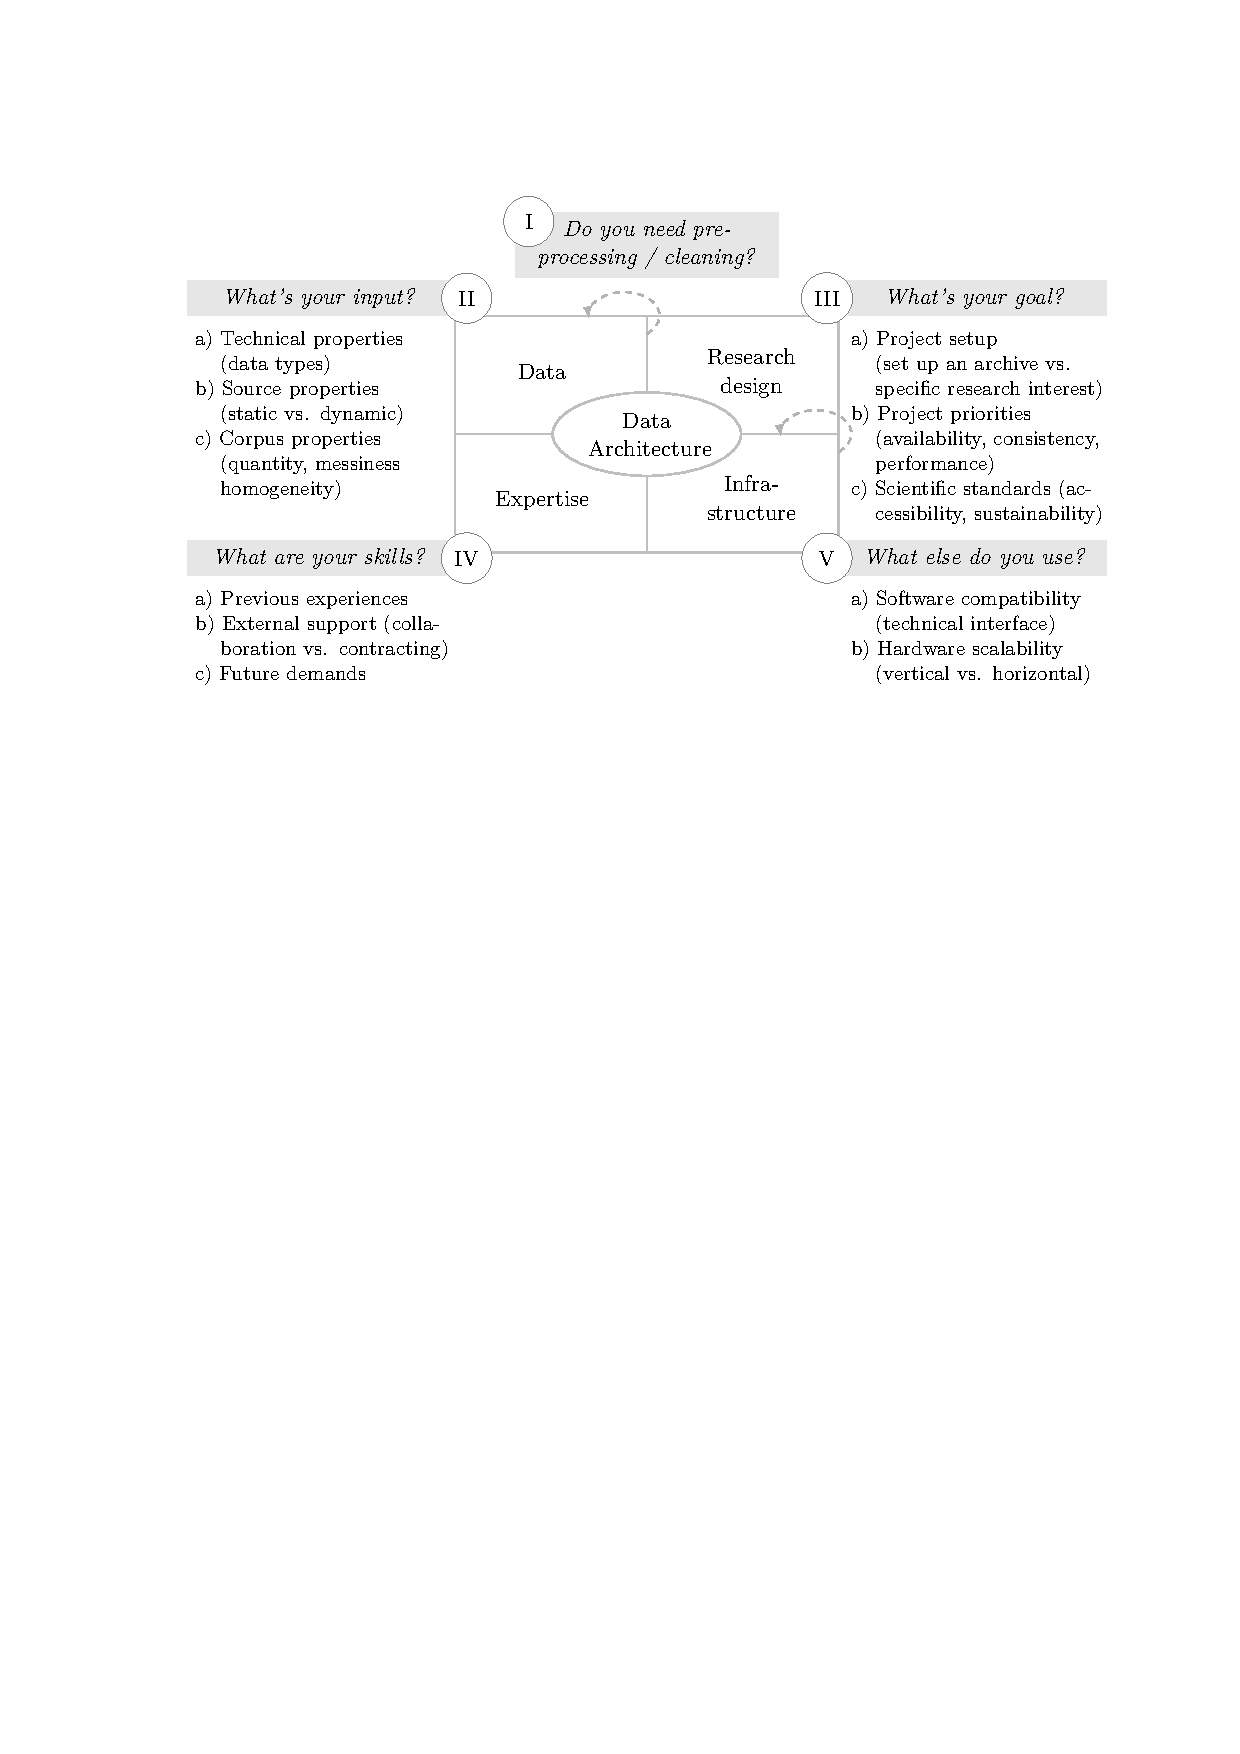
\includegraphics[width=\paperwidth,height=\paperheight,keepaspectratio]{fig2}
	}
\end{frame}




\section{Data architecture}

\begin{frame}[plain]
	Data architecture
\end{frame}

\begin{frame}{Data architecture}
	
	\begin{itemize}
		\item File formats
		\item Linkage
		\item Internal structure
	\end{itemize}
\end{frame}


\begin{frame}
	\makebox[\linewidth]{
		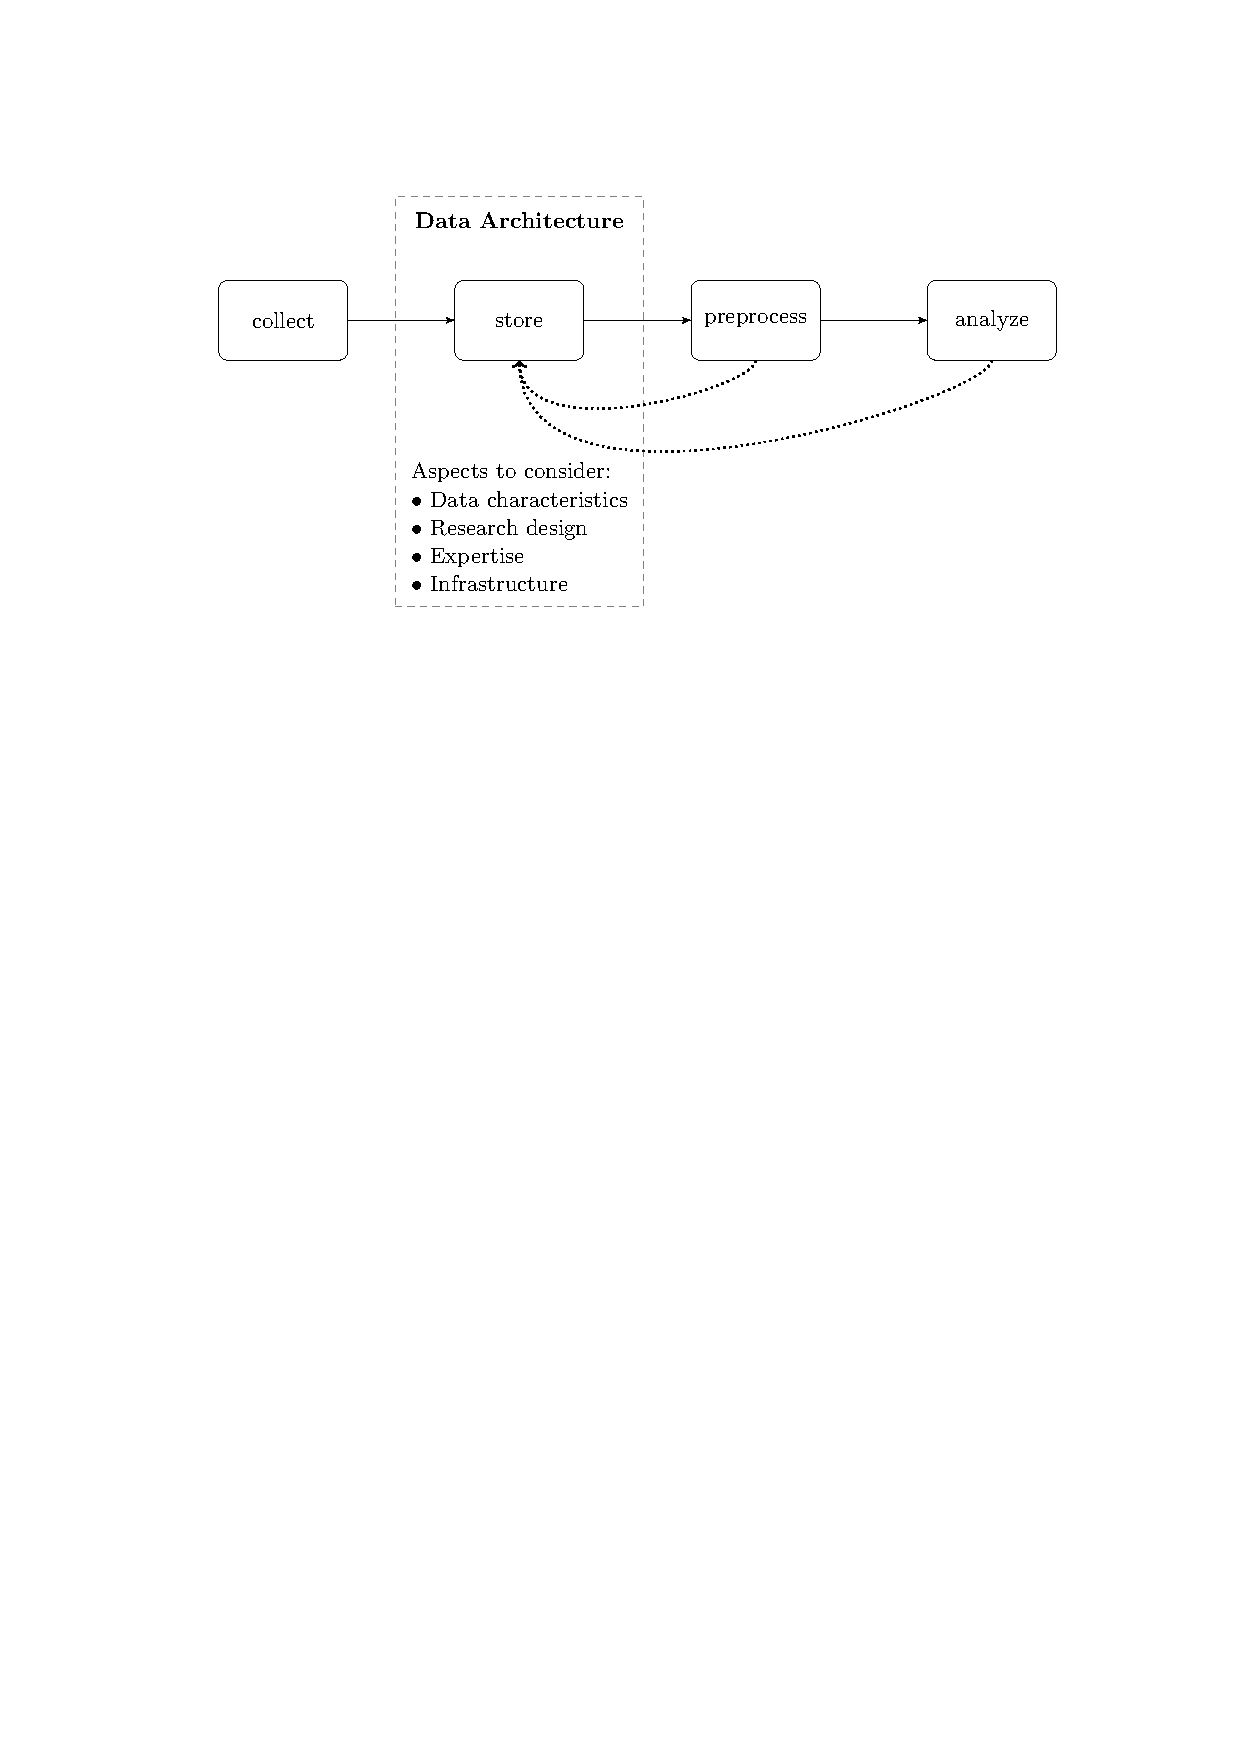
\includegraphics[width=\paperwidth,height=\paperheight,keepaspectratio]{fig1}
	}
\end{frame}





\section{Database types}

\begin{frame}[plain]
	Database types
\end{frame}

\begin{frame}[plain]
	Database types
\end{frame}

\subsection{Relational databases}

\begin{frame}[<+->]{Relational databases}
	\begin{itemize}
		\item Tabular data structure
		\item Relational: tables are linked by keys
		\item Well-defined data types per column
		\item Good at joining and aggregating
	\end{itemize}
\end{frame}


\begin{frame}
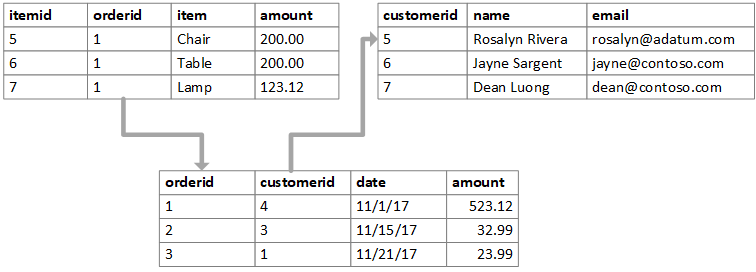
\includegraphics[width=\columnwidth,height=\paperheight,keepaspectratio]{example-relational2}
\end{frame}


\begin{frame}[<+->]{Relational databases and text}
	\begin{itemize}
		\item You can store text
		\item In fact, often used as backend for for instance tweets and sometimes news articles
		\item BUT (1): Not optimized for searching in text
		\item BUT (2): Not good for messy data
		\item BUT (3): Hard to add extra columns or change specifications of existing ones
	\end{itemize}
\end{frame}



\subsection{NoSQL databases}

\begin{frame}[<+->]{NoSQL databases}
	\begin{itemize}
		\item optimized for messy data
		\item can be schema-free $\Rightarrow$ we do not have to enforce a specific format at insertation time 
		\item new entries do not necessarily have to follow the specifications of old ones
		\item Allow you to just throw in an arbitrary JSON object
		\item CAP-theorem: we trade consistency for availability and performance
	\end{itemize}
\end{frame}



\begin{frame}
	We can store retrieved web pages (1) together with some first roughly parsed extracted data (2), and do some cleaning and enrichment (3,4) later.
	\makebox[\linewidth]{
		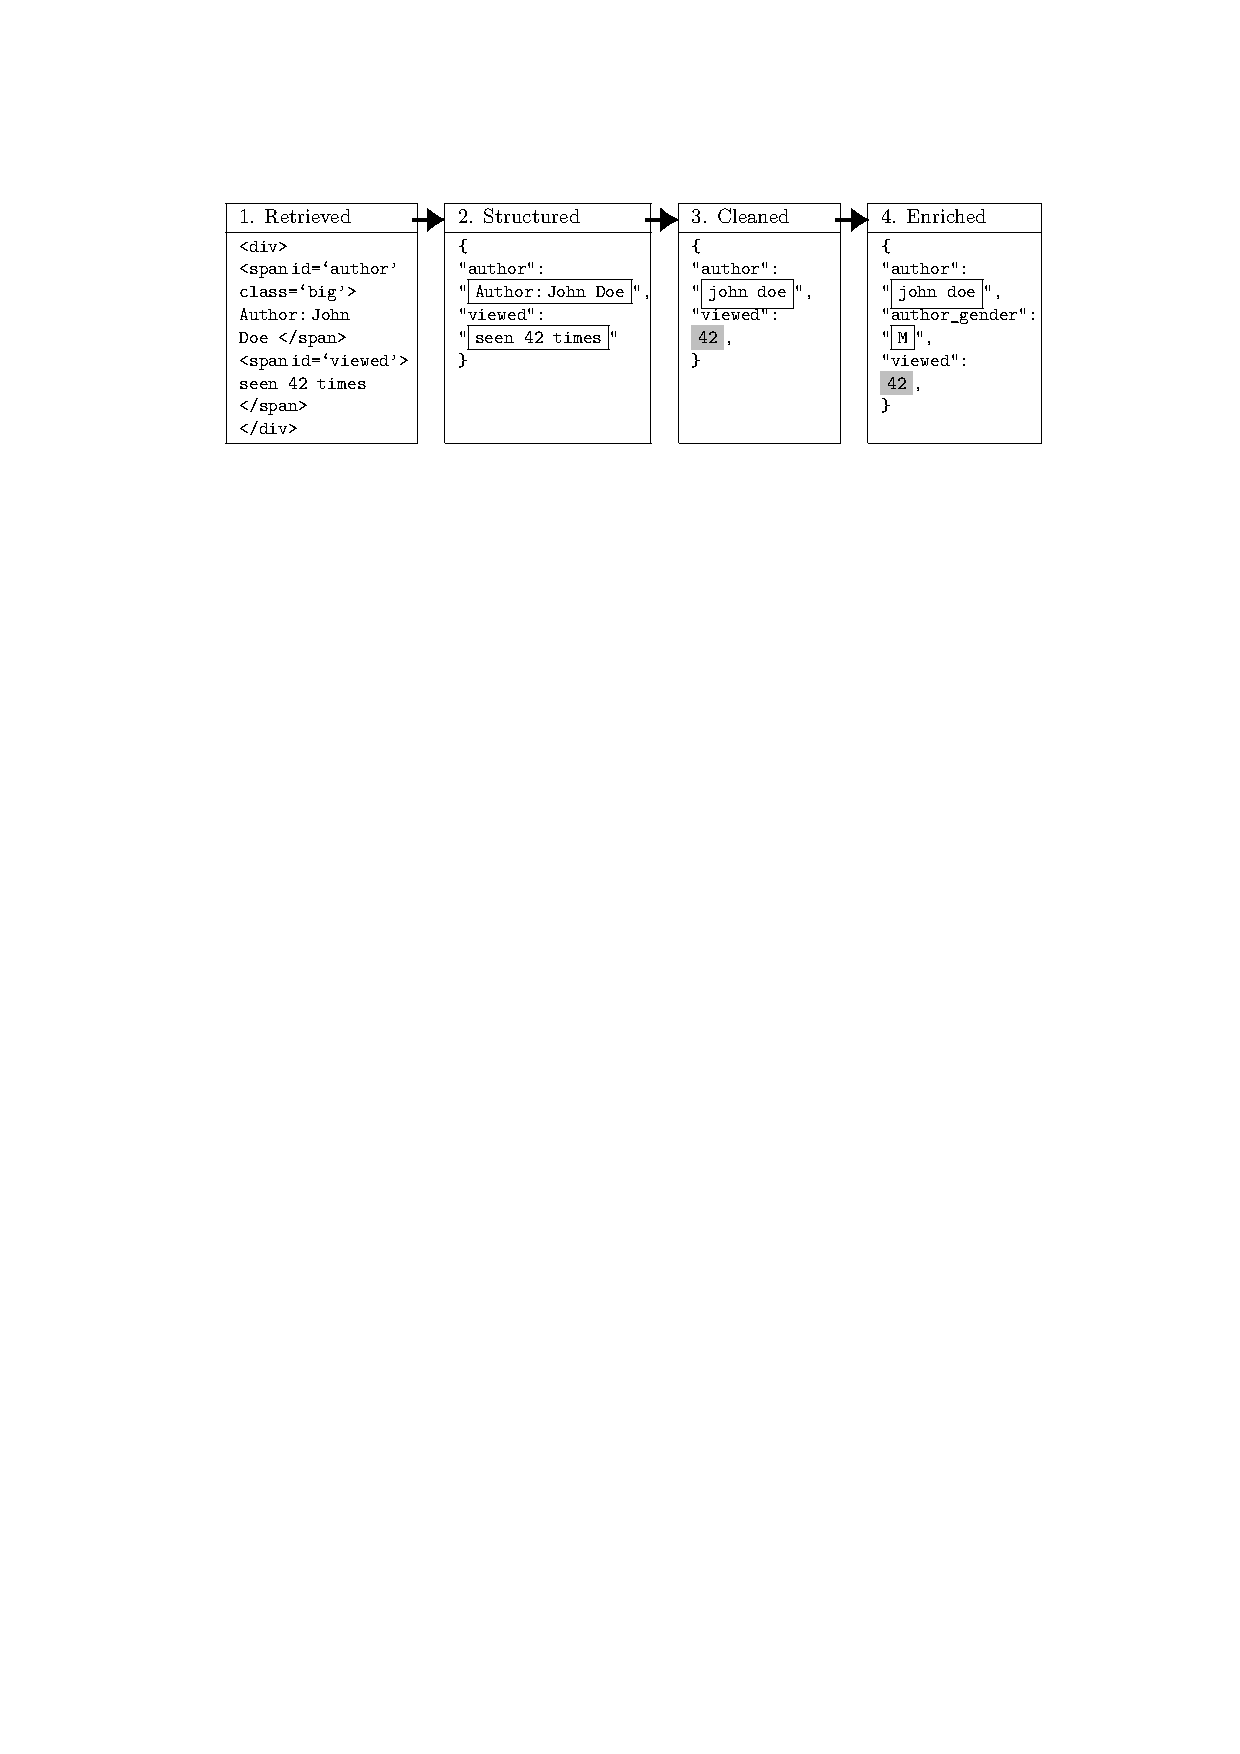
\includegraphics[width=\paperwidth,height=\paperheight,keepaspectratio]{fig3}
	}
\end{frame}



\begin{frame}[<+->]{NoSQL databases and text}
	\begin{itemize}
		\item Often optimized for indexing text
		\item Internal preprocessing (``analysis'') under the hood: e.g., search based on stemmed text
		\item Nested data: e.g., comments within articles
		\item Texts can have additional keys that others don't (e.g., online news have urls, offline news have page numbers; some may have)
		\item You may have even different language versions of the same text (and all having analyzed accordingly)
	\end{itemize}
\end{frame}



\begin{frame}%{SQL vs NoSQL in one slide}
%(for storing (textual) social-scientific data)
\small
\begin{columns}
\column[T]{0.5\linewidth}
\begin{block}{SQL}
	\begin{itemize}
		\item You know the structure in advance
		\item You can differentiate between short strings (e.g., names) stored as VARCHAR and long strings (e.g., articles) stored as TEXT %(TINYTEXT\ldots LONGTEXT) 
		\item You expect that you don't need to query on the TEXTs, which are \emph{not} hold in memory (and need to be fully scanned)
		\item Single source of truth is important, no duplication, consistency to be avoided %(b/c of relational structure)
	\end{itemize}
\end{block}
\pause
\column[T]{0.5\linewidth}
\begin{block}{NoSQL}
		\begin{itemize}
			\item You do not know the (full) structure in advance
			\item Full-text search (including  preprocessed (`analyzed') version ) is relevant
			\item You want to add new keys as you go (e.g., store preprocessing results or enrichments (sentiment scores, predictions))
			\item store first, clean up later
		\end{itemize}
\end{block}
\end{columns}


\end{frame}



\section{MongoDB and Elastic Search}


\begin{frame}[plain]
	MongoDB and Elastic Search
\end{frame}


\begin{frame}[<+->]{Our use case}
	\begin{itemize}
		\item Scrape and store articles ($\approx$ 20M)
		\item We first used Mongo and later switched to ES (because of better performance for full-text search)
		\item On the other hand, there are some who say MongoDB is `safer' (less risk of data loss)
	\end{itemize}
\end{frame}


\begin{frame}{Interacting with ES via http requests}
	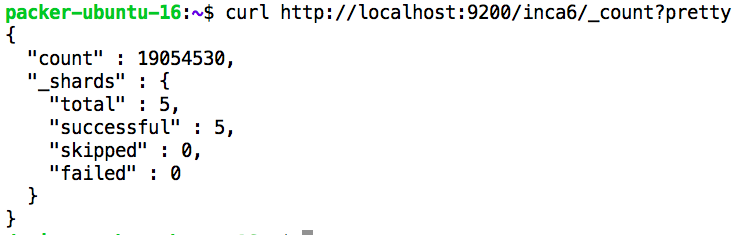
\includegraphics[width=\columnwidth,height=\paperheight,keepaspectratio]{curl}
\end{frame}


\begin{frame}{Interacting with ES via Kibana}
	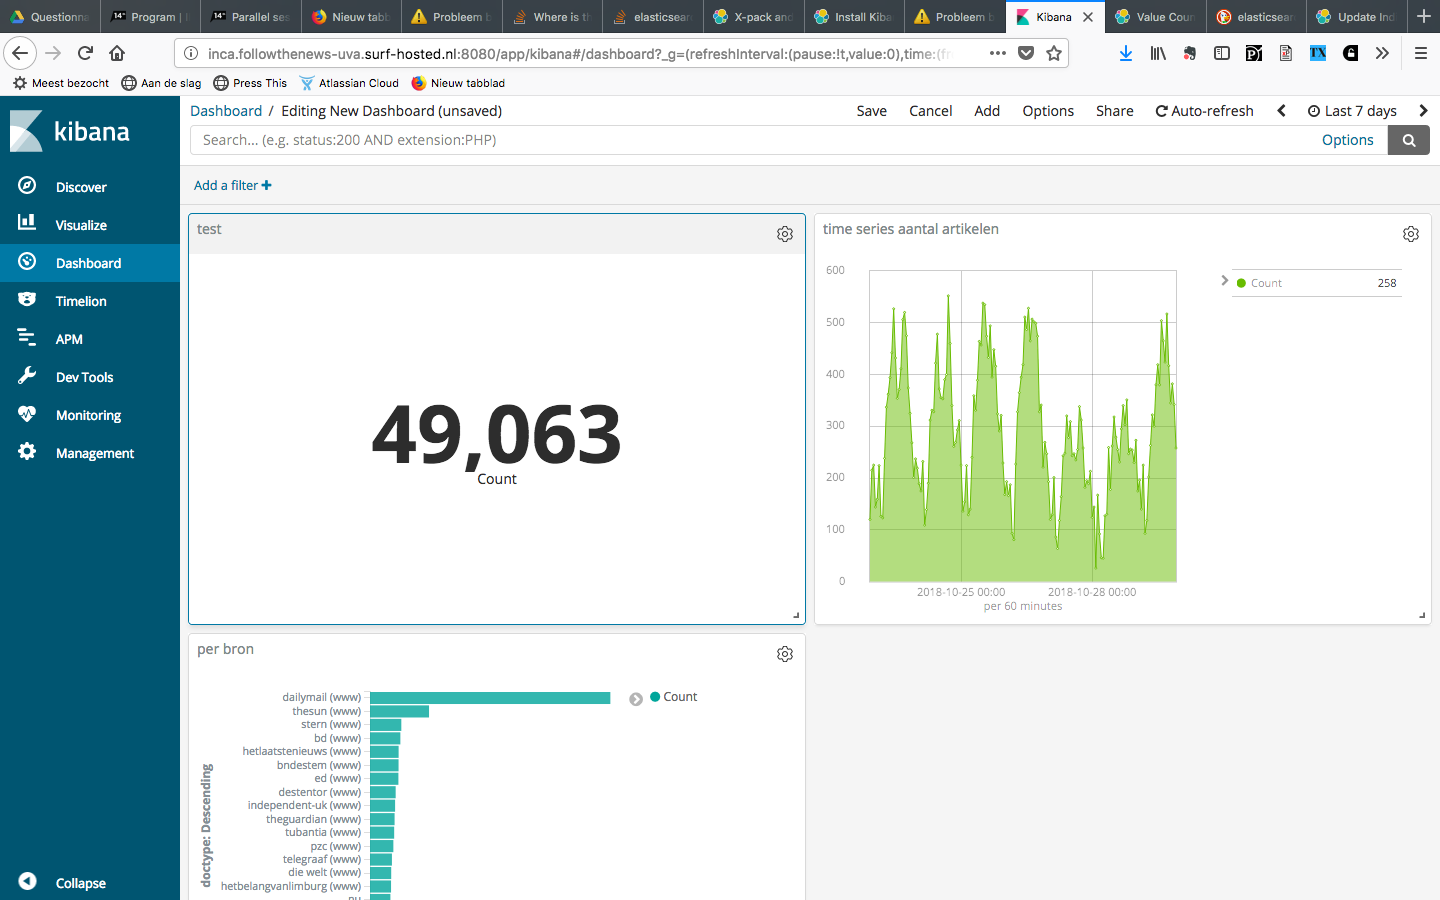
\includegraphics[width=\columnwidth,height=\paperheight,keepaspectratio]{kibana}
\end{frame}


\begin{frame}{Interacting with ES via Python}
	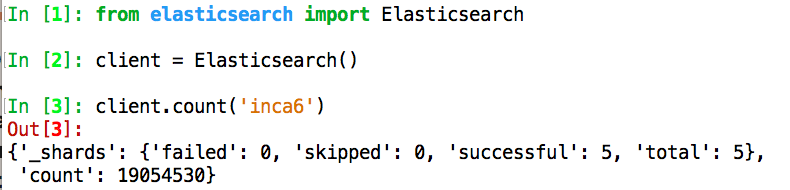
\includegraphics[width=\columnwidth,height=\paperheight,keepaspectratio]{python}
\end{frame}




\section{Practical example}

\begin{frame}
	Practical example (Jupyter Notebook)
\end{frame}

\begin{frame}{Questions?}
\huge
\centering

d.c.trilling@uva.nl

@damian0604

www.damiantrilling.net


	
\end{frame}



\end{document}












